\chapter{Classificação de Tipo de Superfície de Pista 1}
\label{cap:classificacao_tipo_superficie_1}

Nesta seção é apresentado o primeiro de dois estudos voltados ao desenvolvimento de um modelo adaptativo para classificação do tipo da superfície de pista. Este estudo teve como objetivo experimentar e comparar modelos baseados em algumas das técnicas mais utilizadas nos estudos relacionados, com modelos baseados em \textit{Deep Learning}. O processo de desenvolvimento e experimentação é detalhado nas próximas subseções. Na primeira delas, o pré-processamento, foi realizada a seleção de variáveis, normalização dos sinais, extração de características e separação de dados para treinamento e validação. O \textit{design} experimental foi produzido de forma a construir experimentos que permitiram avaliar a capacidade de generalização do aprendizado de cada modelo para contextos desconhecidos e, portanto, avaliar sua adaptabilidade. Na segunda subseção, processamento, foram desenvolvidos e testados 34 diferentes modelos para classificar a superfície de pista, dentre modelos de Aprendizado de Máquina clássico e \textit{Deep Learning}. Por fim, na última subseção são detalhados e comparados os resultados obtidos. 

\section{Pré-Processamento}

Com os conjuntos de dados criados, os dados brutos foram pré-processados antes de serem entregues aos modelos de Aprendizado de Máquina. Este estudo teve como foco a utilização dos valores amostrados no braço de controle, localizado abaixo e próximo ao sistema de suspensão. De acordo com o modelo QC, esses valores possuem interferência apenas da massa não suspensa por meio da rigidez e absorção do pneu \cite{Yafeai2019}. Sendo assim, cada amostra utilizada possuí os valores de força de aceleração e de taxa de rotação, ambos em três eixos, e o valor da velocidade. Neste estudo, utilizamos de ambos os sensores inercias uma vez que os consideramos complementares, com cada um deles fornecendo um tipo específico de dado acerca dos movimentos veiculares. Também consideramos todos os eixos dos sensores e não apenas o de maior interesse, como geralmente é feito nos estudos de exterocepção, uma vez que todos os eixos apresentam informações relevantes, que devem ser consideradas no desenvolvimento de um modelo mais confiável.

Após a seleção das sete variáveis, seus dados foram transformados para se adequar às entradas das técnicas de classificação de padrões. Para os modelos de Aprendizado de Máquina clássicos, foi necessário extrair em pré-processamento as características de alto nível que bem representem as classes de dados. Para isto, foram aplicados os métodos estatísticos Desvio Padrão, Média e Variância para sinais de sensores inerciais e Média para velocidade, os quais constituem os métodos mais comumente usados em estudos relacionados para extrair características baseadas em vibração de sinais de sensores inerciais \cite{Alqudah2016,Andria2016,BelloSalau2018,Bose2018,Hou2017,Li2016,Lima2016,Pholprasit2015,Prapulla2017,Savera2016,Singh2017}. Para os modelos baseados em \textit{Deep Learning}, uma vez que estas técnicas produzem melhor desempenho quando as variáveis são escaladas em uma faixa de valores, os dados foram normalizados com \textit{Robust Scaler}, \textit{Min Max Scaler} no intervalo [0,1] e \textit{Min Max Scaler} no intervalo [-1,1]. Para analisar a influência do número de amostras em todos os modelos, foram criados os \emph{experimentos por tamanho de janela}, onde foram utilizadas janelas fixas de 100, 150, 200, 250 e 300 amostras, considerando 100 o tamanho mínimo para ter informação suficiente, e 300 o tamanho máximo para que o atraso da primeira classificação seja não superior a 3 segundos. 

Após a transformação dos dados, definiu-se quais foram utilizados para treinamento e para validação. Embora um mesmo conjunto de dados seja comumente dividido em uma parte para treinamento e outra para validação (geralmente 70\% - 30\%), ou os conjuntos de dados sejam aplicados em uma metodologia de validação cruzada \textit{k-fold}, ambas as abordagens no contexto deste estudo incorrem em viés por duas razões. A primeira, se todos os conjuntos de dados possuírem uma parte para treinamento e outra para validação ou sejam distribuídos na abordagem \textit{k-fold} de k igual a 9, isso implica que a técnica de reconhecimento de padrões terá para treinamento dados amostrados em todos os veículos, com todos os motoristas, e em todos os cenários. Isso, por si só, já leva a técnica a obter excelentes resultados, mas não nos diz nada sobre a capacidade de generalizar seu aprendizado de classificar padrões em contextos desconhecidos. A segunda razão decorre de que esse tipo de divisão pode levar a situações em que os dados de validação são compostos principalmente por dados com padrões mais facilmente reconhecidos, como segmentos de pavimento asfáltico, uma vez que a vibração do sinal neste tipo de superfície é muito menor do que nas outras. Portanto, para avaliar corretamente a generalização de cada técnica, avaliando sua confiabilidade em contextos desconhecidos (diferentes veículos, motoristas ou cenários/ambientes), os dados de treinamento e validação foram divididos de acordo com o conjunto de dados, separando-os em três \emph{experimentos por contexto}:

\begin{description}
	
	\item[Experimento por Contexto 1:] O modelo aprende dados de todos os veículos e motoristas para alguns cenários; mas não todos os veículos com todos os motoristas para todos os cenários.
    \begin{itemize}
        \item \textbf{Treinamento (65\%):} PVS 1, PVS 3, PVS 4, PVS 6, PVS 7, PVS 9. 
        \item \textbf{Validação (35\%):} PVS 2, PVS 5, PVS 8.
    \end{itemize}
    
    \item[Experimento por Contexto 2:] O modelo aprende dados de todos os cenários para alguns veículos e alguns motoristas; mas não todos os veículos com todos os motoristas para todos os cenários.
    \begin{itemize}
        \item \textbf{Treinamento (66\%):} PVS 1, PVS 2, PVS 3, PVS 7, PVS 8, PVS 9.
        \item \textbf{Validação (34\%):} PVS 4, PVS 5, PVS 6.
    \end{itemize}
    
    \item[Experimento por Contexto 3:] O modelo aprende dados de alguns veículos com alguns motoristas para alguns cenários; mas não todos os veículos com todos os motoristas para todos os cenários.
    \begin{itemize}
        \item \textbf{Treinamento (66\%):} PVS 1, PVS 2, PVS 4, PVS 6, PVS 8, PVS 9.
        \item \textbf{Validação (34\%):} PVS 3, PVS 5, PVS 7.
    \end{itemize}
    
\end{description}

É importante observar que cada conjunto de dados consiste em um conjunto disjunto de variáveis. Portanto, cada um deles contém dados para todas as variáveis de entrada do modelo (força de aceleração, taxa de rotação e velocidade) e a representação de todas as classes de dados (terra, paralelepípedo e asfalto). O que diferencia um conjunto de outro é o contexto de coleta de dados, onde há variação nas propriedades de dependência. A \autoref{fig:divisao_conjuntos_pvs} ilustra a divisão dos grupos de treinamento e validação de acordo com essas propriedades.

\begin{figure}[h]
  \centering
  \caption{Divisão dos conjuntos de dados PVS em grupos de treinamento e validação.}
  \label{fig:divisao_conjuntos_pvs}
  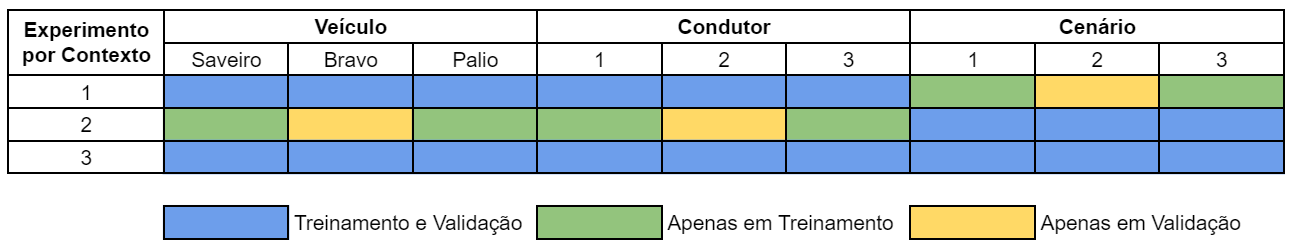
\includegraphics[width=1\textwidth]{figuras/fig_29.png}
  \fonte{Desenvolvido pelo autor.}
\end{figure}

Embora a abordagem de divisão de dados adotada não seja comum, ela foi necessária para permitir avaliar o comportamento dos modelos de Aprendizado de Máquina quando submetido a dados coletados em um veículo, motorista ou cenário desconhecido. Nos três experimentos, todas as classes de dados estão presentes na fase de treinamento e validação. Para avaliar a necessidade de aplicar técnicas de balanceamento de classe de dados, foi medido a distribuição de cada classe conforme detalhado na \autoref{table:distribuicao_classes_tipo_superficie}. A distribuição de classes foi calculada com os dados de treinamento \cite{He2013,Kuhn2013}, uma vez que estes são os dados utilizados pelos modelos para aprender os padrões. A distribuição foi calculada em relação ao número de amostras, uma vez que as janelas de dados são definidas de acordo com esse parâmetro.

\begin{table}[h]
\caption{Distribuição de classes de dados de tipo de superfície de pista.}
\label{table:distribuicao_classes_tipo_superficie}
\centering
\scriptsize
\begin{tabular}{lcccccc}
\cmidrule(l){2-7}
\multicolumn{1}{c}{\multirow{2}{*}{\textbf{}}} & 
\multicolumn{6}{c}{\textbf{Classe de Dados}} \\ \cmidrule(l){2-7} 
\multicolumn{1}{c}{} & 
\multicolumn{2}{c}{\textbf{Terra}} & 
\multicolumn{2}{c}{\textbf{Paralelepípedo}} & 
\multicolumn{2}{c}{\textbf{Asfalto}} \\ \midrule
\textbf{Fonte de Dados} & 
\textit{\textbf{Percentual}} & 
\textit{\textbf{Proporção}} & 
\textit{\textbf{Percentual}} & 
\textit{\textbf{Proporção}} & 
\textit{\textbf{Percentual}} & 
\textit{\textbf{Proporção}} \\ \midrule
% Todos os Conjuntos & 27.69\% & 1:2.6 & 29.07\% & 1:2.4 & 43.23\% & 1:1.3 \\ \midrule
Exp. por Contexto 1 & 21.36\% & 1:3.7 & 36.71\% & 1:1.7 & 41.92\% & 1:1.4 \\ \midrule
Exp. por Contexto 2 & 26.59\% & 1:2.8 & 28.78\% & 1:2.5 & 44.61\% & 1:1.2 \\ \midrule
Exp. por Contexto 3 & 26.15\% & 1:2.8 & 30.26\% & 1:2.3 & 43.58\% & 1:1.3 \\ \bottomrule
\end{tabular}
\fonte{Desenvolvido pelo autor.}
\end{table}

Analisando a \autoref{table:distribuicao_classes_tipo_superficie}, observamos que a distribuição das classes de tipo de superfície de pista situa-se entre 21.36\% e 44.61\%, dependendo do experimento. A proporção varia entre 1:1.2 a 1:3.7, onde para 1 amostra de uma determinada classe de dados, existem de 1.2 a 3.7 amostras nas outras classes. De acordo com \cite{Fernandez2018}, um conjunto de dados é considerado desbalanceado quando existe uma desproporção significativa, ou em alguns casos severa, entre o número de amostras de cada classe. O desbalanceamento de classes pode ser considerado leve ou severo, onde as proporções de distribuição que variam de 1:4 até 1:100 (presença de 20\% - 1\%) são consideradas desbalanceamento leve e proporções de distribuição que variam de 1:100 ou mais (<1\% de presença) são consideradas desbalanceamentos severos \cite{Krawczyk2016,Brownlee2020}. Como podemos observar, as proporções de distribuição das classes de dados neste estudo não é classificada sequer como desbalanceamento leve, pois em seu pior caso, a proporção 1:3.7 ainda é uma distribuição mais uniforme do que 1:4. De acordo com \cite{Brownlee2020}, o desbalanceamento leve geralmente não é uma preocupação, e o problema pode ser tratado como um problema de modelagem preditiva ou classificação normal. Sendo assim, se desbalanceamentos leves não dependem de balanceamento de classes, distribuições mais uniformes, como é o caso deste estudo, certamente não necessitam de aplicação desta técnica.

\section{Processamento}

Após a etapa de pré-processamento, os dados foram utilizados em técnicas de Inteligência Artificial para classificação do tipo de superfície de pista. Por meio de nossa RSL sobre percepção veicular, identificamos as principais técnicas utilizadas na exterocepção veicular com sensores inerciais, a qual tem como objetivo reconhecer as características do ambiente externo como tipo de superfície, qualidade do pavimento, buracos, lombadas, etc. Todos os modelos de Aprendizado de Máquina empregados em estudos anteriores na área são baseados em técnicas clássicas. Portanto, neste estudo foi realizada uma comparação entre as técnicas mais utilizadas na área, todas elas sendo o Aprendizado de Máquina clássico, com as técnicas de Aprendizado Profundo (\textit{Deep Learning}), as quais ainda não foram utilizadas neste tipo de problema de classificação.

Dentre as técnicas de Aprendizado de Máquina clássico mais aplicadas na área, estão as três experimentadas neste estudo: KMC, SVM e KNN. Para a técnica de KMC, foram desenvolvidos modelos com 3 \textit{clusters}, representando as classes a serem agrupadas. Para a técnica de SVM, foram experimentados modelos com três diferentes \textit{kernels}: polinomial de grau 3, rbf e sigmoid. Por fim, para a técnica de KNN, de forma a identificar o valor ótimo de vizinhos, foram desenvolvidos modelos com 1, 2, 5, 10, 50, 100, 250, 500, 1000 vizinhos. No desenvolvimento dos modelos de \textit{Deep Learning}, uma vez que nenhum estudo de exterocepção aplica este tipo de técnica, os modelos produzidos foram baseados em modelos de outros domínios que também utilizam de sensores inerciais para reconhecer padrões. Sendo assim, as Redes Neurais Profundas (\textit{Deep Neural Networks - DNN}) desenvolvidas foram baseadas em estudos de reconhecimento de atividade humana \cite{Deep2019,Alemayoh2019,Chen2015,Yang2018,Zebin2018,Zebin2019,Wang2019,Ahmad2019}, estimativa de velocidade de caminhada \cite{Shrestha2018} e classificação de terrenos durante corrida humana \cite{Dixon2019}. Foram construídos e analisados modelos baseados em LSTM, CNN e CNN-LSTM. Todos os modelos de DNN utilizam o otimizador Adam em conjunto com a função de perda de Entropia Cruzada Categórica, uma vez que se trata de um problema de classificação multi-classe.

Para as redes baseadas em LSTM, vários modelos foram desenvolvidos, dentre \textit{Vanilla} LSTM e \textit{Stacked} LSTM, tanto na forma unidirecional quanto bidirecional, detalhados na \autoref{table:lstm_superficie_pista_1}. O LSTM 7 foi o modelo desenvolvido com melhores resultados, consistindo de uma LSTM \textit{Stacked} Unidirecional detalhada na \autoref{fig:best_lstm_tipo_superficie_1}. Neste modelo, a DNN recebe um tensor de entrada \emph{janelas x sequências x características}, onde \emph{janelas} são os agrupamentos de janelas, \emph{sequências} são os dados que uma janela possui, ou seja, a sequencia de amostras, e \emph{características} são os valores das 7 variáveis dos sensores, sendo assim, os valores de cada amostra. O modelo é composto por uma camada de entrada, três blocos de recorrência e regularização, e um bloco de camadas totalmente conectadas para produção de saída. As camadas de LSTM com 100 unidades são utilizadas para aprender as dependências temporais de longo prazo na sequência de dados. A regularização é feita por duas camadas, sendo \textit{Batch Normalization} para padronizar as entradas de uma nova camada, reduzindo o tempo de treinamento e melhorando o desempenho \cite{Zebin2018}; e \textit{Dropout} em 50\% para evitar \textit{overfitting}, ignorando neurônios selecionados aleatoriamente durante o treinamento. Após o processamento nas camadas recorrentes, os parâmetros são passados para duas camadas \textit{Dense}, a primeira com 100 neurônios com ativação Relu, e a segunda com 3 neurônios e ativação do Softmax, produzindo a classificação. A saída esperada da rede são os rótulos correspondentes à última amostra da janela.

\begin{center}
\scriptsize
\begin{longtable}{cl}
\caption{Modelos de LSTM para classificação do tipo de superfície de pista.}
\label{table:lstm_superficie_pista_1} \\
\toprule 
\multicolumn{1}{l}{\textbf{Nome}} & 
\multicolumn{1}{c}{\textbf{Camadas}} \\ \midrule
\endfirsthead
\toprule 
\multicolumn{1}{l}{\textbf{Nome}} & 
\multicolumn{1}{c}{\textbf{Camadas}} \\ \midrule
\endhead \endfoot \endlastfoot
LSTM 1 & 1 LSTM com 100 unidades, 1 Dropout de 0.5, 1 Dense com 100 unidades e ativação Relu,  1 Dense com 3 \\ & unidades e  ativação Softmax. \\ \midrule
LSTM 2 & Igual a LSTM 1, mas conetando as sequencias \textit{flattened} retornadas pela LSTM diretamente na camada Dense. \\ \midrule
LSTM 3 & Igual a LSTM 1, mas com LSTM bidirecional. \\ \midrule
LSTM 4 & Igual a LSTM 2, mas com LSTM bidirecional. \\ \midrule
LSTM 5 & 3 blocos de LSTM com 100 unidades e Dropout em 0.5, 1 Dense com 100 unidades e ativação Relu, 1 Dense \\ & com 3  unidades e ativação Softmax.\\ \midrule
LSTM 6 & Igual a LSTM 5, mas com LSTM bidirecional e Dropout em 0.2 \\ \midrule
LSTM 7 & 3 blocos de LSTM com 100 unidades, Batch Normalization e Dropout 0.5, 1 Dense com 100 unidades e \\ & ativação Relu, 1 Dense com 3 unidades e ativação Softmax. \\ \bottomrule
\end{longtable}
\fonte{Desenvolvido pelo autor.}
\end{center}

\begin{figure}[h]
  \centering
  \caption{Melhor modelo de LSTM para classificação de superfície de pista.}
  \label{fig:best_lstm_tipo_superficie_1}
  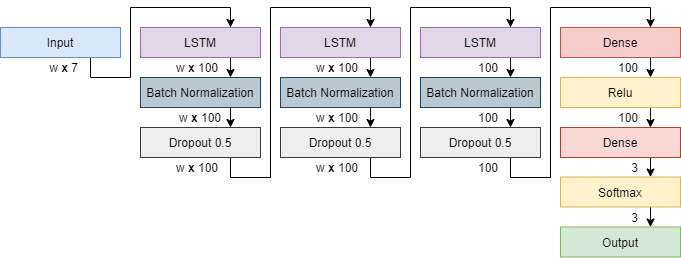
\includegraphics[width=0.8\textwidth]{figuras/fig_31.png}
  \fonte{Desenvolvido pelo autor.}
\end{figure}

Para as redes baseadas em CNN, foram produzidos modelos de CNN \textit{Stacked} utilizando de diferentes camadas de \textit{pooling}, conforme detalha a \autoref{table:cnn_superficie_pista_1}. O modelo desenvolvido com melhores resultados foi o CNN 8, detalhado na \autoref{fig:best_cnn_dnn_tipo_superficie_1}. Esta DNN recebe um tensor de entrada \emph{janelas x sequências x características} semelhante ao das redes baseadas em LSTM, o qual é processado por três blocos de camadas de convolução e regularização, e um bloco de camadas totalmente conectadas. Os blocos de extração de características utilizam nos sinais \textit{kernels} de convolução de tamanho 3, com a primeira camada possuindo 64 filtros e as demais com 32 filtros. A regularização é feita pelas camadas \textit{Batch Normalization} e \textit{Dropout} em 15\% e 20\%. O último bloco de extração de características também possui uma camada \textit{Global Average Pooling 1D} para extrair características mais robustas por valores médios em cada região, acelerando o processo de treinamento e evitando \textit{overfitting} \cite{Yang2018, Wang2019}. Por fim, o último bloco consiste de duas camadas \textit{Dense}, uma com 32 neurônios e ativação de Relu, e a outra com 3 neurônios e ativação de Softmax. A saída esperada da rede são os rótulos mais presentes na janela analisada.

\begin{center}
\scriptsize
\begin{longtable}{cl}
\caption{Modelos de CNN para classificação do tipo de superfície de pista.} 
\label{table:cnn_superficie_pista_1}  \\
\toprule \textbf{Nome} & \multicolumn{1}{c}{\textbf{Camadas}} \\ \midrule
\endfirsthead
\toprule \textbf{Nome} & \multicolumn{1}{c}{\textbf{Camadas}} \\ \midrule
\endhead \endfoot \endlastfoot
CNN 1 &
3 blocos de Conv1D com 64-64-128 filtros, \textit{kernel} de tamanho 3 e ativação Relu, 1 Flatten, 1 Dense com 100 \\ & unidades e ativação Relu, 1 Dense com 3 unidades e ativação Softmax. \\ \midrule
CNN 2 & Igual a CNN 1, mas com 1 Max Pooling 1D com \textit{pool} de tamanho 2 depois dos blocos de convolução. \\ \midrule
CNN 3 & 1 Conv1D com 64 filtros,  \textit{kernel} de tamanho 3 e ativação Relu, 1 Batch Normalization, 1 Dropout em 0.15, \\ & 1 Conv1D com 32 filtros, \textit{kernel} de tamanho 3 e ativação Relu, 1 Global Avg Pool 1D, 1 Batch Normalization, \\ & 1 Dropout 0.2 e 1 Dense com 3 unidades e ativação Softmax.
 \\ \midrule
CNN 4 & 2 Conv1D com 100 filtros, \textit{kernel} de tamanho 10 e ativação Relu, 1 Max Pooling 1D com \textit{pool} de tamanho 3, \\ & 2 Conv1D com 160 filtros, \textit{kernel} de tamanho 10 e ativação Relu, 1 Global Avg Pool 1D, 1 Dropout 0.5 e 1 Dense \\ & com 3 unidades e ativação Softmax.
 \\ \midrule
CNN 5 & 1 Conv1D com 64 filtros, \textit{kernel} de tamanho 3 e ativação Relu, 1 Max Pooling 1D com \textit{pool} de tamanho 2, 1 \\ & Conv1D com 64 filtros, \textit{kernel} de tamanho 3 e ativação Relu, 1 Flatten e 1 Dense com 3 unidades e ativação Softmax.
 \\ \midrule
CNN 6 & 1 Conv1D com 24 filtros, \textit{kernel} de tamanho 8 e ativação Relu, 1 Batch Normalization, 1 Spatial Dropout 0.15, 1 \\ & Conv1D com 12 filtros, \textit{kernel} de tamanho 8 e ativação Relu, 1 Global Avg Pool 1D, 1 Batch Normalization, \\ & 1 Dropout 0.2, 1 Dense com 48 unidades e ativação Relu, 1 Batch Normalization, 1 Dropout em 0.25, 1 Dense com \\ & 3 unidades e ativação Softmax. \\ \midrule
CNN 7 &  3 blocos de Conv1D com 128-64-32 filtros, \textit{kernel} de tamanho 3 e ativação Relu, 1 Batch Normalization e 1 \\ & Max Pooling 1D com \textit{pool} de tamanho 2, 1 Flatten, 1 Dropout em 0.2, 1 Dense com 3 unidades e ativação Softmax. \\ \midrule
CNN 8 & 2 blocos de Conv1D com 64-32 filtros, \textit{kernel} de tamanho 3 e ativação Relu, 1 Batch Normalization e 1 Dropout \\ & em 0.15, 1 Conv1D 32 filtros, \textit{kernel} de tamanho 3 e ativação Relu, 1 Global Avg Pool 1D, 1 Batch Normalization, \\ & 1 Dropout em 0.2, 1 Dense com 32 unidades e ativação Relu e 1 Dense com 3 unidades e ativação Softmax. \\ \bottomrule
\end{longtable}
\fonte{Desenvolvido pelo autor.}
\end{center}

\begin{figure}[H]
  \centering
  \caption{Melhor modelo de CNN para classificação do tipo de superfície de pista.}
  \label{fig:best_cnn_dnn_tipo_superficie_1}
  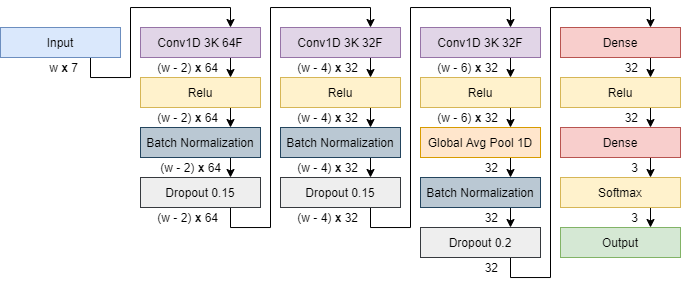
\includegraphics[width=0.8\textwidth]{figuras/fig_32.png}
  \fonte{Desenvolvido pelo autor.}
\end{figure}

Para as redes baseadas em CNN-LSTM, foram produzidos modelos híbridos detalhados na \autoref{table:cnn_lstm_superficie_pista_1}. O modelo desenvolvido com melhores resultados foi o CNN-LSTM 6, detalhado na \autoref{fig:best_cnn_lstm_tipo_superficie_1}. Esta DNN recebe um tensor \emph{janelas x sequências x subsequências x características}, onde \emph{janelas} são os agrupamentos de janelas, \emph{sequências} são as janelas de dados, \emph{subsequências} são os subgrupos de janelas e \emph{características} são os valores das 7 variáveis dos sensores. Os dados são inicialmente processados por três blocos de camadas de convolução e regularização, três blocos de camadas recorrentes e de regularização, e um bloco de camadas totalmente conectadas. Os blocos de extração de características utilizam nos sinais \textit{kernels} de convolução de tamanho 3 com 128 filtros. A regularização é feita pelas camadas de \textit{Batch Normalization} e \textit{Spatial Dropout 1D} em 15\% e 20\%. O último bloco possuí uma camada \textit{Global Average Pooling 1D}. Os blocos recorrentes possuem camadas de LSTM com 100 unidades e regularização por \textit{Batch Normalization} e \textit{Dropout} em 50\%. Finalmente, os parâmetros resultantes são entregues a uma camada \textit{Dense} com 3 neurônios e ativação do Softmax, produzindo a classificação. A saída esperada da rede são os rótulos correspondentes à última amostra na janela.

\begin{center}
\scriptsize
\begin{longtable}{cl}
\caption{Modelos de CNN-LSTM para classificação do tipo de superfície de pista.} 
\label{table:cnn_lstm_superficie_pista_1} \\
\toprule \textbf{Nome} & \multicolumn{1}{c}{\textbf{Camadas}} \\ \midrule
\endfirsthead
\toprule \textbf{Nome} & \multicolumn{1}{c}{\textbf{Camadas}} \\ \midrule
\endhead \endfoot \endlastfoot
CNN-LSTM 1 &  2 Conv1D com 64 filtros, \textit{kernel} de tamanho 3 e ativação Relu, 1 Dropout em 0.5, 1 Max Pooling 1D \\ & com \textit{pool} de tamanho 2, 1 Flatten, 1 LSTM com 100 unidades, 1 Dropout em 0.2, 1 Dense com 100 \\ & unidades e ativação Relu, 1 Dense com 3 unidades e ativação Softmax. \\ \midrule
CNN-LSTM 2 & Igual a CNN-LSTM 1, mas com 3 camadas Conv1D. \\ \midrule
CNN-LSTM 3 & Igual a CNN-LSTM 2, mas com 3 blocos de LSTM e Dropout após a camada Max Pooling 1D. \\ \midrule
CNN-LSTM 4 & Igual a CNN-LSTM 3, mas com os blocos LSTM sem camada Dropout. \\ \midrule
CNN-LSTM 5 &  2 blocos de Conv1D com 128 filtros, \textit{kernel} de tamanho 3 e ativação Relu, Max Pooling 1D com \textit{pool} \\ & de tamanho 2 e Batch Normalization, 1 bloco de 1 Conv1D com 128 filtros, \textit{kernel} de tamanho 3 e ativação \\ & Relu,  Global Avg Pool 1D e Batch Normalization, 3 blocos de 1 LSTM com 100 unidades, Batch \\ & Normalization e Dropout em 0.3, 1 Dense com 3 unidades e ativação Softmax. \\ \midrule
CNN-LSTM 6 & 2 blocos de 1 Conv1D com 128 filtros, \textit{kernel} de tamanho 3 e ativação Relu, Batch Normalization, e Spatial \\ &  Dropout em 0.15, 1 bloco de Conv1D com 128 filtros, \textit{kernel} de tamanho 3 e ativação Relu, Global Avg Pool \\& 1D, Batch Normalization e Dropout em 0.2, 3 blocos de LSTM com 100 unidades, Batch Normalization e \\ & Dropout em 0.3, 1 Dense com 3 unidades e ativação Softmax. \\ \bottomrule
\end{longtable}
\fonte{Desenvolvido pelo autor.}
\end{center}

\begin{figure}[h]
  \centering
  \caption{Melhor modelo de LSTM-CNN para classificação do tipo de superfície de pista.}
  \label{fig:best_cnn_lstm_tipo_superficie_1}
  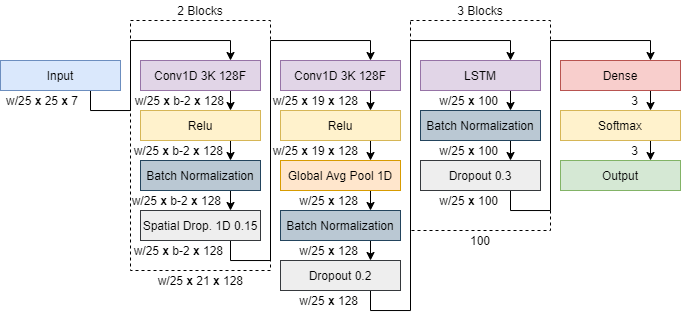
\includegraphics[width=0.8\textwidth]{figuras/fig_33.png}
 \fonte{Desenvolvido pelo autor.}
\end{figure}

\section{Análise de Resultados}

Todos os modelos desenvolvidos neste estudo foram programados em Python 3. Os modelos Aprendizado de Máquina clássico usaram a biblioteca Scikit-Learn, enquanto os modelos \textit{Deep Learning} utilizaram o \textit{framework} Keras com o \textit{backend} Tensorflow. Os experimentos foram realizados no Google Collaboratory, com uma GPU NVIDIA Tesla P100 com 12 GB e 25 GB de RAM. Em todas as técnicas, exceto KNN, os experimentos foram executados 3 vezes a fim de minimizar a aleatoriedade dos parâmetros iniciais, recuperando apenas o melhor entre os três. Cada experimento consiste de um elemento do produto cartesiano entre \emph{experimentos por tamanho de janela} e \emph{experimentos por contexto}. Os resultados obtidos na aplicação do Aprendizado de Máquina clássico são detalhados nas Tabelas \ref{table:kmc_results_tipo_superficie_1}, \ref{table:svm_results_tipo_superficie_1} e \ref{table:knn_results_tipo_superficie_1}. O valor detalhado corresponde à média de acurácia em  validação dos três \textit{experimentos por contexto} para um determinado \emph{experimento por tamanho de janela} e configuração dos hiper-parâmetros da técnica.

\begin{table}[H]
\scriptsize
\centering
\caption{Média de acurácia em validação para os modelos de KMC.} 
\label{table:kmc_results_tipo_superficie_1}
\begin{tabular}{ccccccc}
\cmidrule(lr){2-6}
& \multicolumn{5}{c}{\textbf{Experimentos por Tamanho de Janela}} & \multicolumn{1}{c}{} \\ \midrule
\textbf{Clusters} & \textbf{100} & \textbf{150} & \textbf{200} & \textbf{250} & \textbf{300} & \textbf{Média} \\ \midrule
3 & 56.20\% & 58.13\% &  59.10\% & 59.67\% & \cellcolor[HTML]{34FF34}\textbf{60.42\%} & 58.70\% \\ \bottomrule
\end{tabular}
\fonte{Desenvolvido pelo autor.}
\end{table}

\begin{table}[H]
\scriptsize
\centering
\caption{Média de acurácia em validação para os modelos de SVM.} 
\label{table:svm_results_tipo_superficie_1}
\begin{tabular}{ccccccc}
\cmidrule(lr){2-6}
& \multicolumn{5}{c}{\textbf{Experimentos por Tamanho de Janela}} & \multicolumn{1}{c}{} \\ \midrule
\textbf{Kernel} & \textbf{100} & \textbf{150} & \textbf{200} & \textbf{250} & \textbf{300} & \textbf{Média} \\ \midrule
poly 3 & 65.00\% & 66.60\% & 68.05\% & 68.07\% & \textbf{68.71\%} & 67.28\% \\ \midrule
rbf & 71.95\% & 72.28\% & \cellcolor[HTML]{34FF34}\textbf{72.68\%} & 72.42\% & 72.45\% & 72.36\% \\ \midrule
sigmoid & 52.80\% & 47.08\% & \textbf{57.50\%} & 54.73\% & 56.75\% & 53.77\% \\ \midrule
\textbf{Média} & 63.25\% & 61.99\% & 66.08\% & 65.08\% & 65.97\% & 64.47\% \\ \bottomrule
\end{tabular}
\fonte{Desenvolvido pelo autor.}
\end{table}

\begin{table}[H]
\scriptsize
\centering
\caption{Média de acurácia em validação para os modelos de KNN.} 
\label{table:knn_results_tipo_superficie_1}
\begin{tabular}{ccccccc}
\cmidrule(lr){2-6}
& \multicolumn{5}{c}{\textbf{Experimentos por Tamanho de Janela}} & \multicolumn{1}{c}{} \\ \midrule
\textbf{Vizinhos} & \textbf{100} & \textbf{150} & \textbf{200} & \textbf{250} & \textbf{300} & \textbf{Média} \\ \midrule
1 & 72.28\% & 72.77\% & \textbf{74.46\%} & 73.45\% & 73.83\% & 73.36\% \\ \midrule
2 & 59.80\% & 61.08\% & \textbf{62.69\%} & 60.87\% & 61.92\% & 61.27\% \\ \midrule
5 & 72.37\% & 72.78\% & \cellcolor[HTML]{34FF34}\textbf{74.79\%} & 73.80\% & 73.97\% & 73.54\% \\ \midrule
10 & 67.97\% & 68.39\% & \textbf{70.23\%} & 68.81\% & 69.72\% & 69.02\% \\ \midrule
50 & 70.83\% & 71.54\% & \textbf{72.01\%} & 71.30\% & 69.66\% & 71.07\% \\ \midrule
100 & 69.40\% & \textbf{69.75\%} & 69.47\% & 68.77\% & 67.63\% & 69.00\% \\ \midrule
250 & \textbf{66.25\%} & 65.18\% & 63.84\% & 62.61\% & 61.24\% & 63.83\%\\ \midrule
500 & \textbf{62.15\%} & 59.57\% & 57.66\% & 54.65\% & 53.93\% & 57.59\% \\ \midrule
1000 & \textbf{54.93\%} & 51.42\% & 49.12\% & 45.83\% & 44.05\% & 49.07\% \\ \midrule
\textbf{Média} & 66.22\% & 65.83\% & 66.03\% & 64.45\% & 63.99\% & 65.31\% \\ \bottomrule
\end{tabular}
\fonte{Desenvolvido pelo autor.}
\end{table}

Para a técnica KMC, o melhor modelo resultante para 3 \textit{clusters} foi o de janela com 300 amostras, atingindo 58.24\% de acurácia em treinamento e 60.42\% em validação. Nessa técnica, quanto maior a janela de dados aplicada, maiores os valores de acurácia obtidos. Na técnica SVM, o \textit{kernel} sigmoid obteve os piores valores de acurácia para todas as janelas de dados, seguido pelo \textit{kernel} polinomial de grau 3. Sendo assim, o \textit{kernel} rbf obteve os melhores valores de acurácia para todas as variações de tamanho de janela, onde o modelo com 200 amostras obteve acurácia de 76.15\% para treinamento e 72.68\% para validação. Neste \textit{kernel}, o tamanho da janela de dados tem pouca influência no resultado final. Por fim, os modelos de KNN apresentaram melhores resultados com o número de vizinhos entre 1-50, onde o tamanho da janela também não tem muita influência no resultado. Com grande número de vizinhos, os resultados tendem a apresentar uma variação maior de acordo com o número de amostras na janela. Para o número de vizinhos entre 1-50, a janela com 200 amostras apresentou os melhores resultados, situando o melhor modelo com 5 vizinhos, onde obteve acurácia no conjunto de dados de treinamento de 85.90\% e 74.79\% na validação. Com esses resultados, os melhores modelos de cada técnica clássica são detalhados na \autoref{table:classical_ml_results_tipo_superficie_1}, separados por \emph{experimento por contexto}.

\begin{table}[H]
\scriptsize
\centering
\caption{Valores de acurácia para os melhores modelos baseados em técnicas clássicas de aprendizado de máquina.} 
\label{table:classical_ml_results_tipo_superficie_1}
\begin{tabular}{clcccc}
\cmidrule(lr){3-5}
& & \multicolumn{3}{c}{\textbf{Experimentos por Contexto}} & \multicolumn{1}{c}{} \\ \midrule
\textbf{Modelo} & \multicolumn{1}{c}{\textbf{Fase}} & \textbf{1} & \textbf{2} & \textbf{3} & \textbf{Média} \\ \midrule
\multirow{2}{*}{KMC} & Treinamento & 60.53\% & 56.04\% & 58.13\% & 58.24\% \\ \cmidrule(l){2-6} 
 & Validação & 65.67\% & 60.32\% & 55.26\% & 60.42\% \\ \midrule
\multirow{2}{*}{SVM} & Treinamento & 75.59\% & 77.03\% & 75.84\% & 76.15\% \\ \cmidrule(l){2-6} 
 & Validação & 67.28\% & 75.61\% & 75.16\% & 72.68\% \\ \midrule
\multirow{2}{*}{KNN} & Treinamento & 84.50\% & 86.44\% & 86.76\% & 85.90\% \\ \cmidrule(l){2-6} 
 & Validação & 76.28\% & 71.11\% & 76.98\% & \cellcolor[HTML]{34FF34}\textbf{74.79\%} \\ \bottomrule
\end{tabular}
\fonte{Desenvolvido pelo autor.}
\end{table}

Observando os resultados da Tabela \ref{table:classical_ml_results_tipo_superficie_1}, é possível perceber que a técnica de KNN não somente apresenta a maior média de acurácia, como também é a técnica mais estável, com menor variação de resultado entre experimentos com diferentes contextos. O KMC apresenta variância de 18.07\%, o SVM de 14.63\%, e o KNN de 6.85\%. Além disso, observando a matriz confusão dos melhores modelos na \autoref{fig:confusion_matrix_classical_tipo_superficie_1}, a KNN é a única técnica em que o melhor modelo possuí mais VP e VN que FP e FN, quando considerado cada tipo de superfície separadamente. Sendo assim, conforme detalhado na \autoref{table:classical_ml_metrics_tipo_superficie_1}, KNN tem os melhores valores para f1-score para duas das três classes de dados, classificando segmentos de terra com f1-score de 65.39\%, paralelepípedos com 53.65\% e asfalto com 95.97\%. 

\begin{figure}[H]
  \centering
  \caption{Matriz de confusão para cada melhor modelo de técnicas clássicas de aprendizado de máquina.}
  \label{fig:confusion_matrix_classical_tipo_superficie_1}
  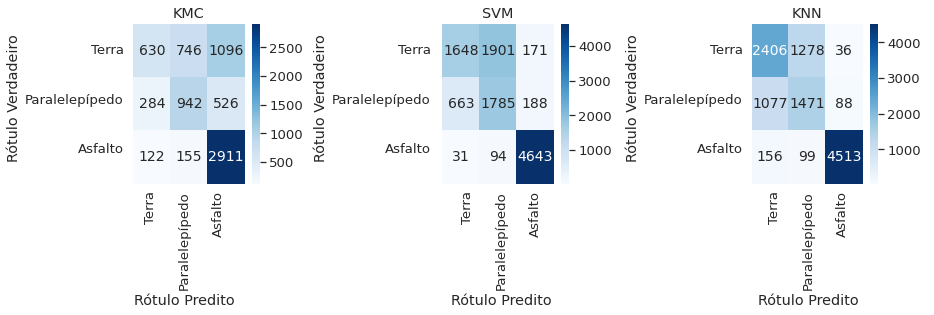
\includegraphics[width=1\textwidth]{figuras/fig_34.png}
  \fonte{Desenvolvido pelo autor.}
\end{figure}

\begin{table}[H]
\scriptsize
\centering
\caption{Métricas de avaliação para cada melhor modelo baseado em técnicas clássicas de aprendizado de máquina.} 
\label{table:classical_ml_metrics_tipo_superficie_1}
\begin{tabular}{clccc}
\toprule
\textbf{Modelo} & \multicolumn{1}{c}{\textbf{Classe de Dados}} & \textbf{F1-Score} & \textbf{Precisão} & \textbf{Recall} \\ \midrule
\multirow{4}{*}{KMC} & Asfalto & 75.40\% & 64.22\% & 91.31\% \\ \cmidrule(l){2-5} 
 & Paralelepípedo & 52.41\% & 51.11\% & 53.77\% \\ \cmidrule(l){2-5} 
 & Terra & 35.92\% & 60.81\% & 25.49\% \\ \midrule
\multirow{4}{*}{SVM} & Asfalto & 95.05\% & 92.82\% & 97.38\% \\ \cmidrule(l){2-5} 
 & Paralelepípedo & 55.64\% & 47.22\% & 67.71\% \\ \cmidrule(l){2-5} 
 & Terra & 54.37\% & 70.37\% & 44.30\% \\ \midrule
\multirow{4}{*}{KNN} & Asfalto & 95.97\% & 97.33\% & 94.65\% \\ \cmidrule(l){2-5} 
 & Paralelepípedo & 53.65\% & 51.65\% & 55.80\% \\ \cmidrule(l){2-5} 
 & Terra & 65.39\% & 66.12\% & 64.68\% \\ \bottomrule
\end{tabular}
\fonte{Desenvolvido pelo autor.}
\end{table}

Para os experimentos com as técnicas de \textit{Deep Learning}, inicialmente foram avaliados os diferentes métodos para normalização dos sinais. Dentre os três experimentados, o \textit{Min Max Scaler} entre [0,1] apresentou piores resultados, atingindo um maior valor de perda e uma acurácia menor. O \textit{Robust Scaler} foi o segundo melhor, mantendo o sinal nos dados, mas sem escalar em um intervalo fixo. Por fim, os dados normalizados com \textit{Min Max Scaler} entre [-1,1], mantendo o sinal e escalando em um intervalo fixo, apresentaram convergência mais rápida, menor perda e maior acurácia. Sendo assim, os escaladores que mantêm o sinal obtiveram melhores resultados, uma vez que o sinal é importante neste estudo, indicando a informação de direção e não apenas uma diminuição de valor. Utilizando os dados normalizados, foram experimentados os modelos de redes propostos. Os resultados são detalhados nas Tabelas \ref{table:lstm_results_tipo_superficie_1}, \ref{table:cnn_results_tipo_superficie_1} e \ref{table:cnn_lstm_results_tipo_superficie_1}.

\begin{table}[H]
\scriptsize
\centering
\caption{Média de acurácia em validação para redes baseadas em LSTM.} 
\label{table:lstm_results_tipo_superficie_1}
\begin{tabular}{ccccccc}
\cmidrule(lr){2-6}
& \multicolumn{5}{c}{\textbf{Experimentos por Tamanho de Janela}} & \multicolumn{1}{c}{} \\ \midrule
\textbf{Modelo} & \multicolumn{1}{c}{\textbf{100}} & \multicolumn{1}{c}{\textbf{150}} & \multicolumn{1}{c}{\textbf{200}} & \multicolumn{1}{c}{\textbf{250}} & \multicolumn{1}{c}{\textbf{300}} & \multicolumn{1}{c}{\textbf{Média}} \\ \midrule
LSTM 1 & 89.14\% & 89.44\% & \textbf{89.86\%} & 86.30\% & 87.59\% & 88.47\% \\ \midrule
LSTM 2 & \textbf{87.38\%} & 87.33\% & 86.80\% & 86.26\% & 85.85\% & 86.72\% \\ \midrule
LSTM 3 & 89.11\% & 89.61\% & 89.99\% & 89.21\% & \textbf{90.45\%} & 89.67\% \\ \midrule
LSTM 4 & 87.12\% & \textbf{87.31\%} & 87.07\% & 86.11\% & 86.48\% & 86.82\% \\ \midrule
LSTM 5 & 89.74\% & 89.14\% & 90.15\% & \textbf{90.60\%} & 89.63\% & 89.85\% \\ \midrule
LSTM 6 & 88.66\% & 89.69\% & \textbf{90.41\%} & 88.99\% & 90.88\% & 89.72\% \\ \midrule
LSTM 7 & 90.39\% & 91.37\% & 91.85\% & 92.71\% & \cellcolor[HTML]{34FF34}\textbf{92.73\%} & 91.81\% \\ \midrule
\textbf{Média} & 88.79\% & 89.13\% & 89.45\% & 88.60\% & 89.09\% & 89.01\% \\ \bottomrule
\end{tabular}
\fonte{Desenvolvido pelo autor.}
\end{table}

\begin{table}[H]
\scriptsize
\centering
\caption{Média de acurácia em validação para redes baseadas em CNN.} 
\label{table:cnn_results_tipo_superficie_1}
\begin{tabular}{ccccccc}
\cmidrule(lr){2-6}
& \multicolumn{5}{c}{\textbf{Experimentos por Tamanho de Janela}} & \multicolumn{1}{c}{} \\ \midrule
\textbf{Modelo} & \textbf{100} & \textbf{150} & \textbf{200} & \textbf{250} & \textbf{300} & \textbf{Média} \\ \midrule
CNN 1 & 87.44\% & 87.60\% & \textbf{88.25\%} & 87.07\% & 87.54\% & 87.58\% \\ \midrule
CNN 2 & 87.58\% & 87.82\% & 88.25\% & \textbf{88.65\%} & 87.94\% & 88.05\% \\ \midrule
CNN 3 & 89.98\% & 91.67\% & 92.91\% & 92.81\% & \textbf{93.02\%} & 92.08\% \\ \midrule
CNN 4 & 88.88\% & 90.20\% & 91.13\% & 91.78\% & \textbf{92.00\%} & 90.80\% \\ \midrule
CNN 5 & 86.87\% & 87.71\% & \textbf{88.61\%} & 87.81\% & 88.35\% & 87.87\% \\ \midrule
CNN 6 & 90.09\% & 91.12\% & 91.61\% & \textbf{92.17\%} & 91.94\% & 91.39\% \\ \midrule
CNN 7 & 89.17\% & 89.59\% & \textbf{90.14\%} & 89.66\% & 89.65\% & 89.64\% \\ \midrule
CNN 8 & 91.02\% & 91.83\% & 92.89\% & 92.99\% & \cellcolor[HTML]{34FF34}\textbf{93.17\%} & 92.38\% \\ \midrule
\textbf{Média} & 88.88\% & 89.69\% & 90.47\% & 90.37\% & 90.45\% & 89.97\% \\ \bottomrule
\end{tabular}
\fonte{Desenvolvido pelo autor.}
\end{table}

\begin{table}[H]
\scriptsize
\centering
\caption{Média de acurácia em validação para redes baseadas em CNN-LSTM.} 
\label{table:cnn_lstm_results_tipo_superficie_1}
\begin{tabular}{ccccccc}
\cmidrule(lr){2-6}
& \multicolumn{5}{c}{\textbf{Experimentos por Tamanho de Janela}} & \multicolumn{1}{c}{} \\ \midrule
\textbf{Modelo} & \textbf{100} & \textbf{150} & \textbf{200} & \textbf{250} & \textbf{300} & \textbf{Média} \\ \midrule
CNN-LSTM 1 & 87.56\% & 89.15\% & 89.35\% & \textbf{90.97\%} & 90.78\% & 89.56\% \\ \midrule
CNN-LSTM 2 & 87.92\% & 88.38\% & 89.76\% & 89.54\% & \textbf{90.47\%} & 89.21\% \\ \midrule
CNN-LSTM 3 & 87.45\% & 88.77\% & 90.09\% & 89.79\% & \textbf{91.04\%} & 89.43\% \\ \midrule
CNN-LSTM 4 & 87.43\% & 89.43\% & 89.51\% & 89.93\% & \textbf{90.99\%} & 89.46\% \\ \midrule
CNN-LSTM 5 & 90.03\% & 90.69\% & 91.23\% & 91.54\% & \textbf{92.71\%} & 91.24\% \\ \midrule
CNN-LSTM 6 & 90.27\% & 91.50\% & 92.10\% & 92.48\% &\cellcolor[HTML]{34FF34}\textbf{92.77\%} & 91.82\% \\ \midrule
\textbf{Média} & 88.44\% & 89.65\% & 90.34\% & 90.71\% & 91.46\% & 90.12\% \\ \bottomrule
\end{tabular}
\fonte{Desenvolvido pelo autor.}
\end{table}

Todos os modelos de DNN propostos, mesmo nos piores resultados, apresentaram valores de acurácia em treinamento e validação maiores do que os obtidos pelo melhor modelo baseado em Aprendizado de Máquina clássico. Isso evidencia a capacidade do \textit{Deep Learning} de aprender relações mais complexas entre os dados, em comparação às técnicas clássicas. Em todos os experimentos, o impacto na acurácia dado o tamanho da janela da amostras é praticamente insignificante, enquanto que as técnicas clássicas possuem grande variação. Em todas as abordagens de \textit{Deep Learning} experimentadas, o uso da camada de \textit{Bacth Normalization}, além de acelerar o treinamento, melhorou os resultados em todos as execuções. O uso da camada \textit{Dropout} também se mostrou importante para a generalização do modelo. Nos modelos baseados em LSTM, a utilização de camadas bidirecionais praticamente não alteraram os resultados, tendo aumento de acurácia para algumas janelas, e diminuição para outras, sempre em valores praticamente irrelevantes e, na média, menores que 1\%. O uso de vetores de sequências retornados pela LSTM conectados diretamente nas camadas totalmente conectadas \textit{Dense} piorou os resultados em todos os experimentos, diminuindo o valor de acurácia em até 4\%. Sendo assim, o modelo baseado em LSTM com os melhores resultados é o LSTM 7, em uma janela de 300 amostras, onde atingiu um valor de acurácia em treinamento de 96.67\% e 92.73\% em validação.

Nas redes baseadas em CNN, a utilização de duas a quatro camadas de convolução se mostrou essencial para extração das características. Na saída final dos blocos de convolução para conexão com o bloco de camadas totalmente conectadas, a utilização de \textit{pooling} melhorou os resultados quando comparado ao uso de apenas \textit{flattening}. Tanto a camada \textit{Max Pooling} quanto a \textit{Global Average Pooling} melhoraram os resultados, com a segunda sendo significativamente melhor. Sendo assim, todos os experimentos nos quais a média de acurácia das janelas foi maior que 90\%, houve a utilização do \textit{Global Average Pooling}. O modelo baseado em CNN com os melhores resultados foi o CNN 8, com uma janela de 300 amostras, atingindo uma acurácia em treinamento de 95.56\% e 93.17\% em validação. Por fim, nas redes híbridas CNN-LSTM as mesmas considerações das baseadas em LSTM e CNN se aplicam, com o melhor modelo sendo a CNN-LSTM 6 com janela de 300 amostras, obtendo acurácia em treinamento de 94.9\% e de 92.77\% em validação. Os melhores modelos para cada abordagem de \textit{Deep Learning} são detalhados na \autoref{table:deep_ml_results_tipo_superficie_1}.

\begin{table}[H]
\scriptsize
\centering
\caption{Valores de acurácia para os melhores modelos baseados em técnicas \textit{deep learning}.} 
\label{table:deep_ml_results_tipo_superficie_1}
\begin{tabular}{clcccc}
\cmidrule(lr){3-5}
& & \multicolumn{3}{c}{\textbf{Experimentos por Contexto}} & \multicolumn{1}{c}{} \\ \midrule
\textbf{Modelo} & \multicolumn{1}{c}{\textbf{Fase}} & \textbf{1} & \textbf{2} & \textbf{3} & \textbf{Média} \\ \midrule
\multirow{2}{*}{LSTM} & Treinamento & 98.54\% & 98.45\% & 93.03\% & 96.67\% \\ \cmidrule(l){2-6} 
 & Validação & 93.60\% & 91.88\% & 92.70\% & 92.73\% \\ \midrule
\multirow{2}{*}{CNN} & Treinamento & 94.39\% & 97.62\% & 94.67\% & 95.56\% \\ \cmidrule(l){2-6} 
 & Validação & 94.93\% & 92.25\% & 92.33\% & \cellcolor[HTML]{34FF34}\textbf{93.17\%} \\ \midrule
\multirow{2}{*}{CNN-LSTM} & Treinamento & 91.68\% & 98.85\% & 94.16\% & 94.90\% \\ \cmidrule(l){2-6} 
 & Validação & 93.68\% & 92.67\% & 91.97\% & 92.77\% \\ \bottomrule
\end{tabular}
\fonte{Desenvolvido pelo autor.}
\end{table}

\begin{figure}[H]
  \centering
  \caption{Matriz de confusão para cada melhor modelo de técnicas de \textit{deep learning}.}
  \label{fig:confusion_matrix_deep_tipo_superficie_1}
  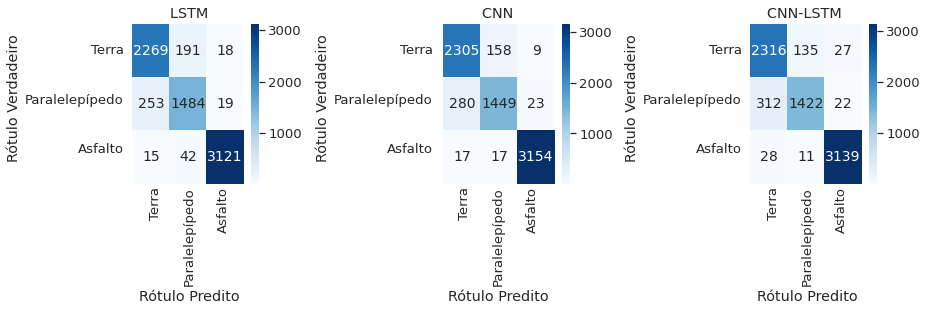
\includegraphics[width=1\textwidth]{figuras/fig_35.png}
  \fonte{Desenvolvido pelo autor.}
\end{figure}

\begin{table}[H]
\scriptsize
\centering
\caption{Métricas de avaliação para cada melhor modelo baseado em técnicas de \textit{deep learning}.} 
\label{table:deep_ml_metrics_tipo_superficie_1}
\begin{tabular}{clccc}
\toprule
\textbf{Modelo} & \multicolumn{1}{c}{\textbf{Classe de Dados}} & \textbf{F1-Score} & \textbf{Precisão} & \textbf{Recall} \\ \midrule
\multirow{4}{*}{LSTM} & Asfalto & 98.52\% & 98.83\% & 98.21\% \\ \cmidrule(l){2-5} 
 & Paralelepípedo & 85.46\% & 86.43\% & 84.51\% \\ \cmidrule(l){2-5} 
 & Terra & 90.49\% & 89.44\% & 91.57\% \\ \midrule
\multirow{4}{*}{CNN} & Asfalto & 98.96\% & 99.00\% & 98.93\% \\ \cmidrule(l){2-5} 
 & Paralelepípedo & 85.84\% & 89.23\% & 82.71\% \\ \cmidrule(l){2-5} 
 & Terra & 90.85\% & 88.59\% & 93.24\% \\ \midrule
\multirow{4}{*}{CNN-LSTM} & Asfalto & 98.62\% & 98.46\% & 98.77\% \\ \cmidrule(l){2-5} 
 & Paralelepípedo & 85.56\% & 90.69\% & 80.98\% \\ \cmidrule(l){2-5} 
 & Terra & 90.22\% & 87.20\% & 93.46\% \\ \bottomrule
\end{tabular}
\fonte{Desenvolvido pelo autor.}
\end{table}

Com base na \autoref{table:deep_ml_results_tipo_superficie_1}, é possível observar que as diferentes abordagens de \textit{Deep Learning} se mostraram adequadas para o problema de classificação proposto. Avaliando a média de acurácia em validação, o modelo baseado em CNN foi ligeiramente melhor do que os outros, embora o baseado em LSTM foi o melhor no experimento 3, o baseado em CNN melhor no experimento 1, e o baseado em CNN-LSTM melhor no experimento 2. Analisando a matriz de confusão na \autoref{fig:confusion_matrix_deep_tipo_superficie_1} e outras métricas de avaliação detalhadas na \autoref{table:deep_ml_metrics_tipo_superficie_1}, observamos que o modelo baseado em CNN tem os maiores valores de f1-score para todas as classes de dados, sendo o melhor modelo quando se considera não apenas sua capacidade de obter VP e VN, mas também de evitar FP e FN. Portanto, consideramos o modelo de CNN como o melhor modelo baseado em \textit{Deep Learning} para a classificação do tipo de superfície de pista devido a sua maior acurácia e valores de f1-score, além de ser o modelo com menor custo computacional entre os três modelos DNN. Sendo assim, a técnica obteve um valor de acurácia na validação de 93.17\%, classificando estrada de terra com valor f1-score de 90.85\%, paralelepípedo com 85.84\% e asfalto com 98.9\%, obtendo resultados melhores que os métodos clássicos e que os estudos relacionados, aplicando ainda variações contextuais.
